%!TEX root = ../../../ECP-ST-CAR.tex 

\subsubsection{\stid{5.10} ExaWorks} \label{subsubsect:exaworks}

% ECP ST Project Overviews: A significant portion of this report includes 2-page synopses of each
% ECP ST project (Section 4), including a project overview, key challenges, solution strategy, recent progress and next steps

\paragraph{Overview} 
Exascale computers will offer transformative capabilities to combine
data-driven and learning-based approaches with traditional simulation
applications to accelerate scientific discovery and insight. These software
combinations and integrations, however, are difficult to achieve due to
challenges of coordination and deployment of heterogeneous software components
on diverse and massive platforms. The ExaWorks project is addressing 
many of these challenges by co-designing a Software Development Kit (SDK)
consisting of a wide range of workflow management tools that can be
composed and interoperate through common interfaces. 
The project is working to collect an initial
set of tools, design common interfaces supported, make tools
easier to apply to complex science challenges, and develop examplar use cases.
The project is community-centered, embracing the various stakeholders, including
users, developers, and facility representatives, to 
sustainably address the requirements of workflows at
the exascale.




\paragraph{Key Challenges}
Emerging exascale workflows pose significant challenges to the creation of
portable, repeatable, and performant workflows. These challenges are both
technical and non-technical. On the technical side, workflow management systems (WMSs) are currently
incapable of supporting the needs of heterogeneous co-scheduled and
high-throughput workflows, as well as enabling communication between fine
grain tasks in dynamic workflows. On the non-technical side, the myriad WMSs
that exist, lack of reusable WMS components, and the absence  of clear user
guidance when selecting a WMS has resulted in a disjoint workflows community
that tends toward building ad hoc or bespoke solutions rather than adopting
and extending existing solutions.

Specific challenges include: 
\begin{enumerate}
    \item Workflows community: the workflows, applications, and facility communities are disjoint. 
    Efforts are needed to bring these groups together to agree on common workflow components and interfaces, 
    and to work together to develop, integrate, and support these components.
    \item Scheduling: exascale workflows must manage the efficient execution of diverse
    tasks (e.g., in runtime, resource requirements, single/multi-node) with complex interdependencies on increasingly heterogeneous resources. 
    \item Scale and performance: emerging workflows feature huge ensembles of short-running jobs, 
    which can create millions or even billions of tasks that need to be rapidly scheduled and executed.
    \item Coordination and communication: workflows depend on coordination between the workflow and 
    the tasks within the workflow, a need that requires efficient exchange of data following various communication patterns.
    \item Fault tolerance: the enormous number of computing elements and workflow tasks increases 
    the likelihood of encountering faults within a workflow both at the system level and also from the millions of concurrent tasks. 
    \item Portability: most WMSs are tested on a handful of systems and the frequency by which
    system hardware and software change makes it impossible to guarantee that a workflow will work on even the same system in the future.
\end{enumerate}

\paragraph{Solution Strategy}
The ExaWorks project lays the foundation for an inherently
\textit{new approach} to workflows: establishing an SDK (see
Figure~\ref{fig:arch}) by assembling components from existing workflow
projects and defining new component interfaces. The ExaWorks SDK provides a robust, well-tested, documented,
and scalable set of tools and components that can be combined to enable diverse teams to
produce scalable and portable workflows for a wide range of exascale
applications. Importantly, the project is not creating a new workflow system
nor does it aim not to replace the many workflow solutions already deployed
and used by scientists, but rather it will provide well engineered and
scalable SDK which can be leveraged by new and existing workflows.


\begin{wrapfigure}[15]{r}{0.5\textwidth}
\begin{center}
    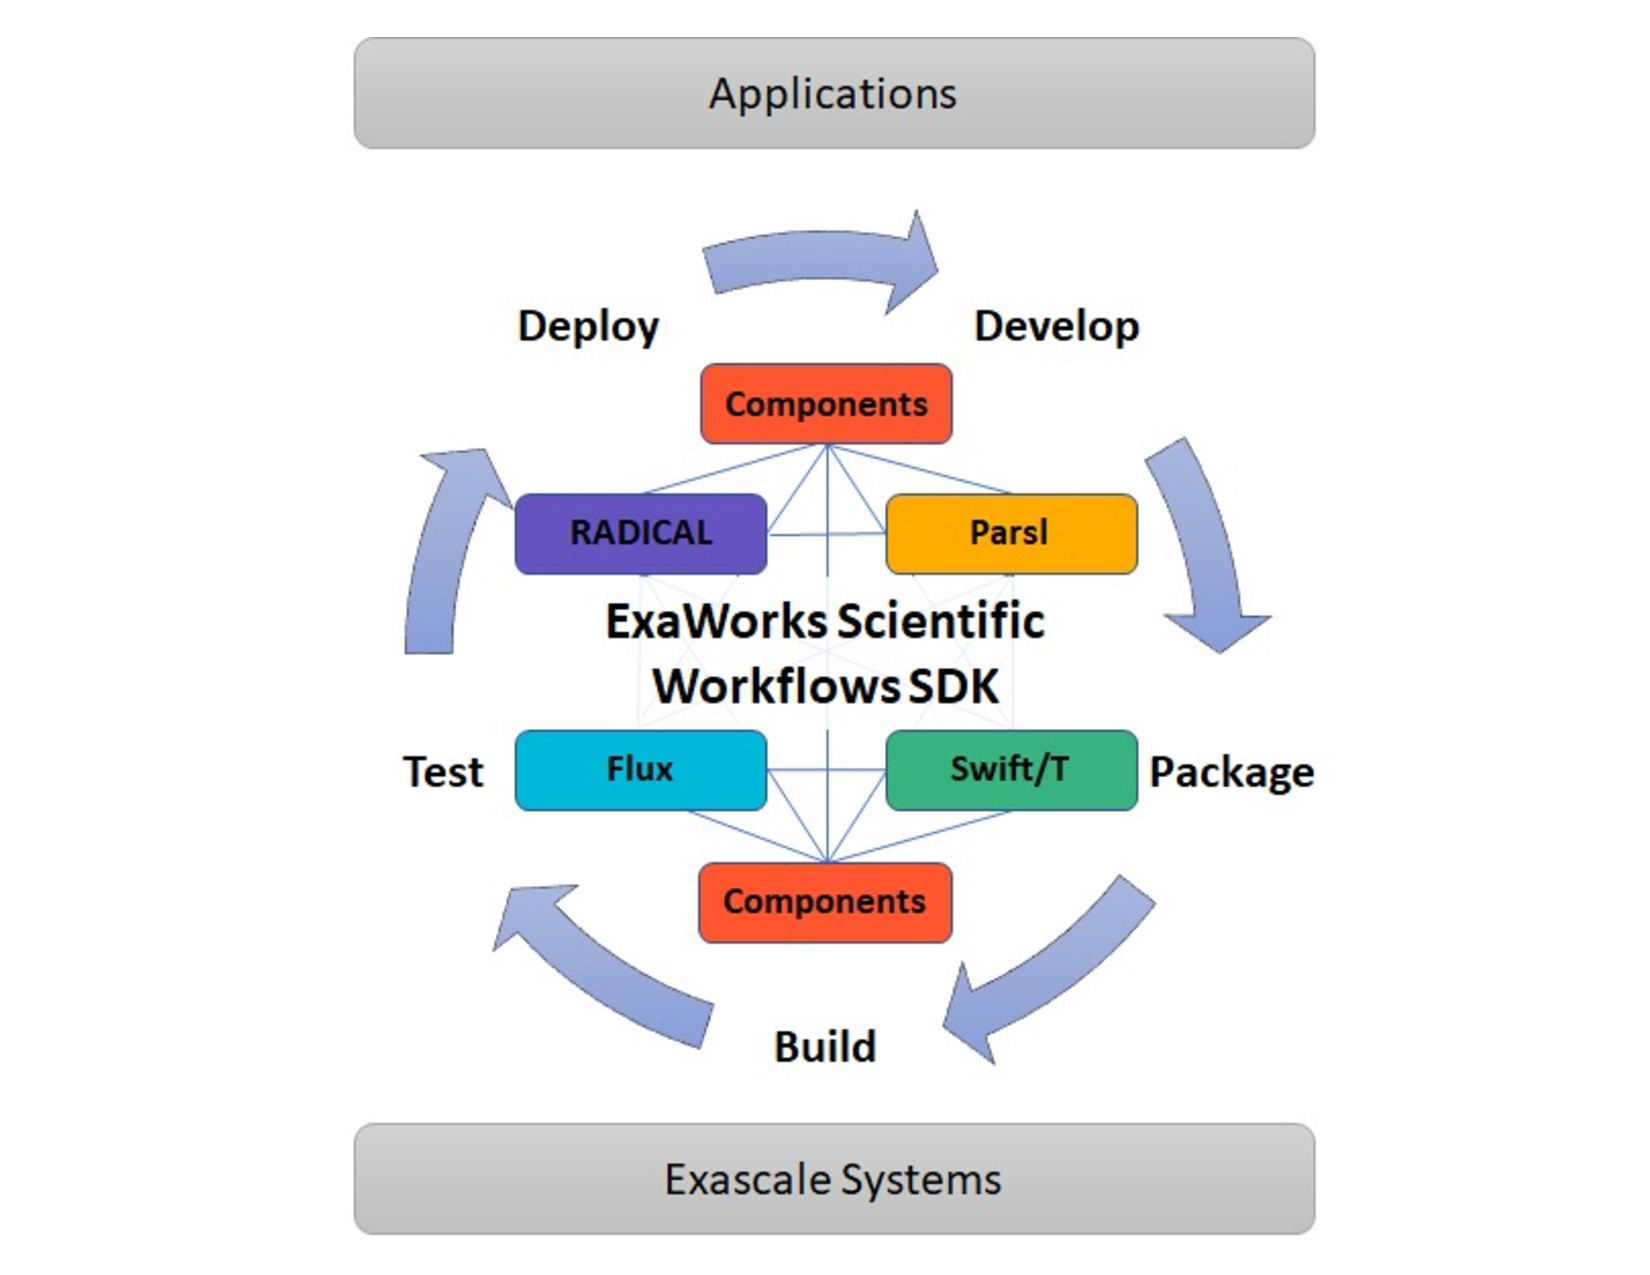
\includegraphics[width=0.5\textwidth]{projects/2.3.5-Ecosystem/2.3.5.10-ExaWorks/ExaWorks_Circle.pdf}
  \end{center}
  \caption{ExaWorks Toolkit\label{fig:arch}}
\end{wrapfigure} 

The goals of the first year of the project are to instantiate the ExaWorks SDK, seeding it with
robust workflow components, explore pairwise-integrations between components, and define
common component interfaces for shared components.  The project also aims to impact ECP applicaitons and 
bring together the workflows community, including developers, ECP applications, and DOE compute facility representatives
to collectively address workflows challenges.
%.  Specifically, it will:
% \begin{enumerate}
%     \item Engage the facilities to survey the state of workflow tools and capabilities and ways in which ExaWorks can enhance their capabilities;
%     \item Establish an advisory board composed of representatives of DOE compute facilities, ECP applications, and workflow tools, to guide and advise ExaWorks;
%     \item Survey ECP applications teams to identify the tools currently being used and to identify common challenges and needs;
%     \item Assemble a functional design working group to develop a community-centered draft function design; and
%     \item Collaborate with ECP applications to develop a proof-of-concept integration using a shared functional component as defined by the draft design, in an ECP application.
% \end{enumerate}

\paragraph{Recent Progress}
% In this period of the project we have
% assembled our advisory committee, 
% started a functional design working group, and distributed a workflows
% survey to the ECP community. The results of this survey are helping
% to prioritize in-person interviews as well as informing the 
% functional design process and helping to identify initial ExaWorks components. 
% Our team have started prototyping efforts to explore 
% component-based approaches in existing workflow systems. Specifically, 
% we have developed prototype Balsam and RADICAL-Pilot executors for Parsl
% which enable Parsl workflows to leverage the resource management 
% capabilities of these external systems.



In this period of the project have focused on instantiating the SDK, defining and developing
the first component interface, working with ECP applicaiton teams, and engaging
the workflows community. We breifly describe efforts in each area. 

We released the first version of the ExaWorks SDK, after first defining
community policies~\cite{sdk-policies} (modeled on E4S) and developing continuous integration and packaging
approaches. We have seeeded the SDK with five workflow technologies 
that are widely used in ECP applicaitons. We followed a community-based
approach in which all artifacts are tracked using an open process on GitHub.
Our packaging solutions allow for portable and reproducible deployment and 
testing techniques, which vary considerably among workflow tools.  
We have defined a Fork+Pull model-based GitHub development workflow and and 
GitHub Actions-based continuous integration testing and deployment for SDK components.

Following a community-based approach, we identified our first component interface for
the SDK: PSI/J, a portability layer across different HPC workload managers 
allowing workflow developers and users to create portable workflows with a standard API. 
%Our survey highlighted the challenge of porting workflows as one of the most critical needs for workflow developers and users alike. 
PSI/J is composed of both a language-agnostic community-defined specification~\cite{jpsi-spec} and the 
specification's language-specific implementations. 
As a community, we have focused initially on implementing a PSI/J Python 
library~\cite{jpsi-python}.   The Python library contains the set of
core classes defined by the specification, as well as abstract base classes (ABCs) for components 
that implement functionality specific to different clusters and batch systems.
The implementation currently supports Slurm, LSF, Cobalt, RADICAL-Pilot, and Flux connectors. 

We have continued to impact ExaLearn and CANDLE through ongoing
collaborations, and have strengthened collaborations with the ExaAM team. The
ExaAM workflow is composed of several application codes, each capturing a
different scale or physics of the problem.  Each stage feeds
information to the next stage, and iteration can occur across stages.  Some
stages leverage CPU's and others GPU's. Several stages are themselves small
workflows typically leveraging the \textit{ensemble} motif. Thus, the ExaAM
workflow requires integration of multiple physics applications and when
executed at full scale will require complex orchestration of many
sub-workflows.  The ExaAM collaboration provides a strong vehicle for co-design and informing the 
ExaWorks SDK. Initial integration of ExaWorks SDK technologies has shown that
improvements in throughput are possible with minor changes to existing scripts.
The ExaAM and ExaWorks teams have identified additional stages in the workflow
that could benefit by incrementally integrating ExaWorks SDK capabilities to
improve portability and performance.  In order to facilitate this engagement,
the ExaAM team has produced an example workflow capability of being executed
upon ECP CI infrastructure and that will be used to demonstrate integration of additional
ExaWorks SDK components.

In collaboration with the NSF-funded WorkflowsRI project, we are hosting
a series of workflows community summits that aim to bring the diverse
workflows community together. 
The first summit brought together 48 international participants representing many WMSs, 
with the goal to identify crucial challenges in the workflows community. 
The summit considered six broad themes: FAIR workflows, training and education,
AI workflows, exascale challenges, APIs and interoperability, and developing workflow community. 
The second summit~\cite{summit_2} focused on technical approaches for realizing 
many of the challenges identified in the first summit. It included 75 workflows developers %from around the world
and focused on three core topics: 
defining common workflow patterns and benchmarks, identifying paths toward interoperability of workflow systems, and improving workflow systems’ interface with legacy and emerging HPC software and hardware.
We also host an open monthly community meeting that is attended by representatives across
DOE laboratories.



\paragraph{Next Steps}
% The remainder of this initial effort focuses on four important areas. 
% First, continuing to grow the ExaWorks community by engaging with ECP 
% applications, facilities, and WMS teams. 
% Second, working with these partners and stakeholders to produce a draft
% functional design document that outlines ExaWorks components
% and potential interfaces to these components. 
% Third, we will produce a report, derived from interviews from 
% the broad ECP community that outlines ECP workflows needs, challenges, 
% and potential solutions. 
% Finally, we will demonstrate the technical feasibility of the 
% ExaWorks approach via application of preliminary components to
% at least one ECP application. 


The next steps for the SDK are to develop and harden deeper 
integration of our technologies, to extend our CI/CD pipeline to ECP systems,
and to integrate other community workflows tools.
Thus far, we have focused on small-scale interoperation, but we plan to extend our solutions to
ensure scalable integration of the components on pre-exascale and early access exascale
systems for immediate readiness as exascale systems become available.
Finally, we are preparing an SC ExaWorks tutorial which will be a foundational piece of a comprehensive
SDK documentation effort.

For applications engagement, we plan to build on the ExaAM workflow to explore
and showcase multiple SDK technologies, and to boot-strap integrated testing of
the components in a realistic workflow. We will leverage this engagement to
gain real-world experience in how the SDK can be leveraged by application teams
and integrated with CI and other infrastructures.  We also plan to apply our
SDK to ECP applications to address broad workflow needs.
